\phantomsection
\subsubsection*{Հրահանգների համար հարցումներ}\label{subsubsec:instructions}
\addcontentsline{toc}{subsubsection}{Հրահանգների համար հարցումներ}

Այս հարցումները ևս բաժանվում են երկու խմբի`
\begin{enumerate}
    \item հրահանգների որոնման հարցումներ,
    \item հրահանգների վերլուծության հարցումներ:
\end{enumerate}

Օգտագործողները կարող են որոնել հրահանգներն ըստ՝
\begin{enumerate}
    \item տիպի (օրինակ՝ IF, FOR, CALL և այլն),
    \item դասերի,
    \item կանչած ֆունկցիաների և այլն։
\end{enumerate}

Սա թույլ կտա օգտագործողներին արագ և թիրախավորված կերպով գտնել իրենց հետաքրքրող հրահանգները:

Երբ օգտագործողն ընտրել է կոնկրետ հրահանգը, նա կարող է անցնել դրա մանրամասն վերլուծությանը:  Հրահանգների վերլուծության հարցումների
միջոցով հնարավոր կլինի ստանալ տեղեկություններ՝
\begin{enumerate}
    \item նախորդող և հաջորդող հրահանգների մասին,
    \item օպերանդների մասին,
    \item տվյալ հրահանգը պարունակող ֆունկցիայի մասին,
    \item կանչվող ֆունկցիաների մասին և այլն։
\end{enumerate}

\begin{figure}[h]
    \centering
    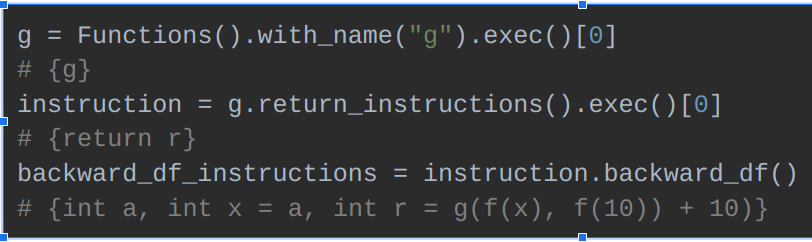
\includegraphics[width=0.7\textwidth]{pic15}
    \caption{Հրահանգների համար հարցումների օրինակ}
    \label{fig:figure15}
\end{figure}

Այսպիսով, հրահանգների համար նախատեսված հարցումները թույլ կտան օգտագործողներին արագ գտնել և մանրամասն վերլուծել
ծրագրի ղեկավարման և տվյալների հոսքերը: Սա կարևոր է ծրագրի արդյունավետության և անվտանգության վերլուծման համար:
